\documentclass{article}
\usepackage[T1]{fontenc}
\usepackage[utf8]{inputenc}
\usepackage[margin=1in]{geometry}
\usepackage{fancyhdr} 
\usepackage{listings}
\usepackage{algorithm}
\usepackage[noend]{algorithmic}
\usepackage{amsmath, amsthm, amssymb, amsfonts}
\usepackage{graphicx}
\usepackage[dvipsnames]{xcolor}
\usepackage{xy}
\usepackage{url}
\usepackage{parskip}
\usepackage{comment}
\usepackage{setspace}
\usepackage{enumerate}
\usepackage{multirow}
\usepackage{hyperref}
\usepackage{caption}
\usepackage{subcaption}
\usepackage{booktabs}
\usepackage{wrapfig}
\usepackage{times}

\captionsetup[figure]{font={small,it}}

\usepackage[backend=biber,style=numeric,sortcites,maxbibnames=99]{biblatex}
\addbibresource{references.bib}

\newcommand{\HRule}{\rule{\linewidth}{0.5mm}}
\newcommand{\Hrule}{\rule{\linewidth}{0.3mm}}
\newcommand{\classnum}{CS-GY 6313 B}

\makeatletter% since there's an at-sign (@) in the command name
\renewcommand{\@maketitle}{%
  \parindent=0pt% don't indent paragraphs in the title block
  \centering
  {\Large \bfseries\textsc{\@title}}
  \HRule\par%
  \textit{\@author \hfill \classnum}
  \par
}
\makeatother% resets the meaning of the at-sign (@)

\title{Assignment 1: What are the average monthly sunshine hours in U.S. cities (1981-2010)?}
\author{Sanyukta Tuti}
% \classnum

\begin{document}
  \maketitle % prints the title block
  \thispagestyle{empty}
  % \vspace{-15pt}

\begin{figure}[ht] % Change the position of your figure https://www.overleaf.com/learn/latex/Positioning_images_and_tables
    \centering
    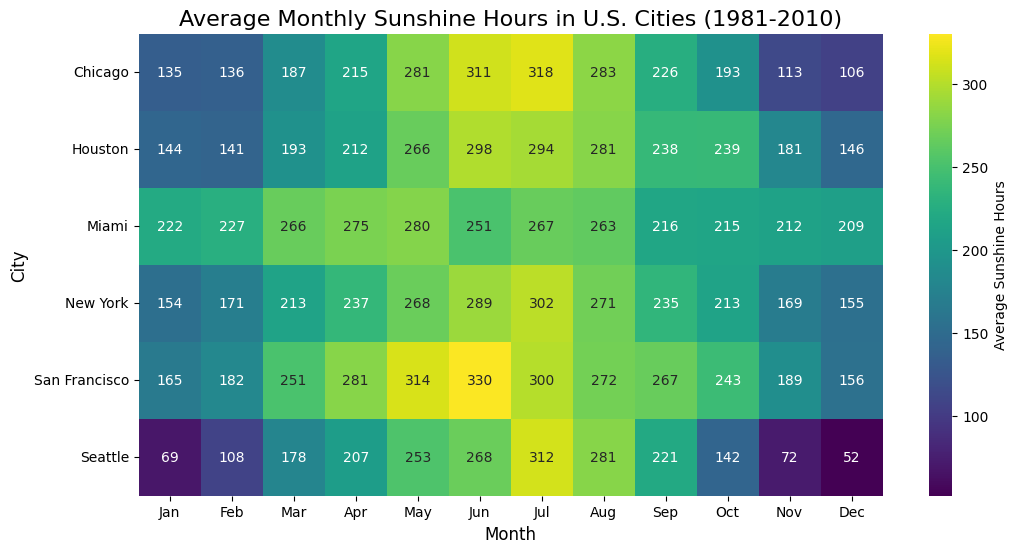
\includegraphics[width=1.0\textwidth]{Information Vsualization/figs/Heatmap.png}
    \caption{
        Heatmap for the Average Monthly Sunshine Hours in U.S. Cities (1981-2010)
    }
    \label{fig:fig1}
\end{figure}

\section{Visualizing Design}
\label{sec:sec1}

During my design process, I experimented with three visualizations: a \textbf{stacked bar plot}, \textbf{line plot}, and \textbf{heatmap}, to address the question, "What are the average monthly sunshine hours in U.S. cities (1981-2010)?" I initially selected the bar chart for comparing sunshine hours between cities and the line plot to highlight seasonal trends. However, I ultimately found the heatmap to be the most effective, as it enables easy comparison of sunshine patterns across both cities and months simultaneously.

\subsection{Rationale Behind Design Choices:}
                
Initially, I created a \textbf{stacked bar plot} that showed the total sunshine hours for each city, with the x-axis representing the months and the y-axis representing the sunshine hours. Although it provided a clear representation of cumulative sunshine, comparing individual months between cities proved difficult, as the stacked format obscured monthly values. Furthermore, while the color coding highlighted the categorical differences between cities using identity channels, it was less effective in showing detailed seasonal variations.\cite{munzner2014visualization}

Next, I experimented with a \textbf{line plot} where each city was represented by a line, and the x-axis represented the months of the year. This visualization highlighted seasonal trends well and made it easier to track each city’s sunshine hours over time. However, it still lacked precision in comparing exact values for each month, and with multiple overlapping lines, it became visually complex.

Finally, I designed a \textbf{heatmap} to visualize the seasonal variations in sunshine hours across six U.S. cities. The heatmap provides a clear, intuitive way to compare sunshine hours across both months and cities using a color gradient to represent the number of sunshine hours. Each row corresponds to a city, and each column represents a month, making it easy to spot geographic and seasonal patterns.
                
\begin{itemize}
    \item \textbf{Color Gradient}: I applied VIRIDIS color palette to represent sunshine hours, leveraging the magnitude channel to reflect the diverging ordered nature of the data. By inverting the colors, lighter shades indicate higher sunshine values, while darker shades represent lower values.  This choice is robust to colorblindness and enhances visual perception, for easy distinction between high and low sunshine periods across cities.\cite{TheComprehensiveRArchiveNetwork}\cite{munzner2014visualization}
                    
    \item \textbf{Annotations}: I annotated sunshine hours directly on the heatmap to provide exact values for each month and city, ensuring that precise comparisons can be made without relying solely on color perception.
                    
    \item \textbf{Labels}: Months are arranged in calendar order along the x-axis, while cities are represented along the y-axis, allowing for a natural reading flow and an intuitive understanding of the data.

    \item \textbf{Size and layout}: The heatmap is meticulously designed for optimal readability, maintaining a suitable aspect ratio and a generous cell spacing to avoid distortion of data representation and enhance perceptual clarity.
\end{itemize}
                
\textbf{Insights:}
\begin{itemize}

    \item \textbf{Miami} and \textbf{Houston} consistently have high sunshine hours throughout the year, with little variation between months, as indicated by lighter cells.
                    
    \item \textbf{Seattle} and \textbf{New York} experience much darker cells during the winter months, showing significantly lower sunshine hours compared to other cities.

    \item The heatmap captures both the geographic variation (north vs. south) and the seasonal variation (summer vs. winter) effectively, revealing trends at a glance.
                    
\end{itemize}

\section{Conclusion}
                
While the heatmap effectively conveys overall trends, it struggles to convey a clear narrative of changes due to its limitations in representing value differences for immediate visual comparison as detailed month-to-month comparisons between cities require careful attention to color perception. Annotations can help alleviate this challenge. Overall, the heatmap strikes a balance between simplicity and precision, addressing the central question of how sunshine differs throughout the year. However, its effectiveness may diminish with larger datasets, as increased density can obscure significant patterns and complicate interpretation.\cite{heatmap}

\newpage

\begin{refcontext}[sorting=nyt]
\printbibliography
\end{refcontext}

\end{document}

